\subsection{iOS}
	Eine Applikation unter iOS kommuniziert wie auch unter Android (Kapitel
	\ref{sec:app-android}) nicht direkt mit  der Hardware sondern mit nativ
	gegebenen Schnittstellen, welche sich zwischen der App und der Hardware
	befinden und wie ein Schichtensystem angesehen werden können. Dabei steigen
	Komplexität, wie auch Nutzungsmöglichkeiten pro hinzukommender Schicht an.
	Durch diese vorgegebene Art der Hardwarenutzung wird ein immer gleich
	bleibender Standard und eine gewisse Einheitlichkeit im Bereich der Entwicklung
	garantiert.
	\begin{figure}[h]
		\centering
		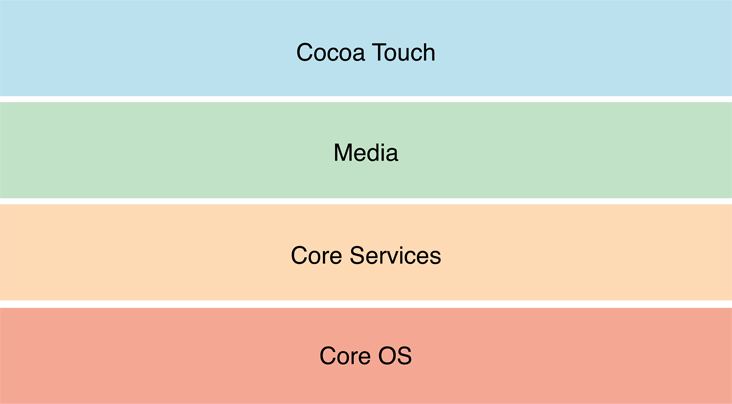
\includegraphics[width=0.5\linewidth]{ios/media/ios-layers.png}
		\caption{Ebenen der iOS Applikationsstruktur
		\cite{AboutiOSTech2015}}
		\label{fig:marcetshare}
	\end{figure}
	\\
	Apps für iOS werden in Objective-C (auch: ObjC) und darunter ansässigen
	Sprachen C++ und C verfasst. Zusätzlich ist seit der Vorstellung von
	\textsl{Swift} auf der Apple Entwicklerkonferenz WWDC im Jahre 2014 eine
	neue hauseigene Sprache dazu gekommen. ObjC ist eine Erweitung von C, welche
	seit dem Erscheinen von Swift immer mehr an Beliebtheit verliert, wohingegen
	Swift seinen Stand bis Juni 2015 im TIOBE-Index deutlich verbessern
	konnte \cite{TIOBE062015}.
	\subsubsection{Struktur}
		Applikationen unterliegen der MVC\footnote{MVC:
		Model-View-Controller}-Architektur, welche Objekten drei verschiedene Rollen
		zuweist und den Umgang dieser untereinander regelt. Die "`Model-Rolle"'
		ummantelt dabei die Daten und stellt Mittel bereit, um auf diese zuzugreifen
		und zu verändern. Die "`View-Rolle"' ist für Darstellung verantwortlich und
		reagiert unter anderem auf Eingaben des Nutzers. Die "`Controller-Rolle"' ist
		der Vermittler zwischen View und Model und kann Einfluss auf den
		\textsl{Lebenszyklus} anderer Objekte nehmen.
	\subsubsection{Entwicklungsumgebung und Lizenzen}
		iOS Apps können nur mit der integrierten Entwicklungsumgebung Xcode
		entwickelt werden. Diese stellt Apple \textsl{OS X Yosemite}
		Benutzern, als auch registrierten Entwicklern kostenlos zur Verfügung.
		Eine Entwicklerlizenz schlägt mit 99 US-Dollar pro Jahr zu Buche. Eine
		Teilnahme am \textsl{iOS Developer Enterprise Program} (vgl. Kapitel
		\ref{sec:appsigning}) kostet Firmen jährlich 299 US-Dollar
		\cite{AppleDev2015}.
	\subsubsection{Technologien zur App-Entwicklung}
		iOS stellt eine Fülle an Bibliotheken bereit, welche von der
		tiefen und hardwarenahen Programmierung abstrahieren. Dies ermöglicht mit
		weniger Programmierarbeit bessere Ergebnisse zu erzielen und eventuell
		komplexe Aufgaben, wie Speicherallokation oder Multithreading an tiefere
		Schichten abzugeben \cite{AboutiOSTech2015}.
		Apple empfiehlt eine Arbeitsweise auf möglichst abstrahierter Ebene.
		Nachfolgend wird auf einzelne Bestandteile dieser Schichtenarchitektur
		eingegangen. Es gilt anzumerken, dass es sich hier um keine vollständige
		Auflistung handelt, da dies den Rahmen dieser Arbeit übersteigen würde.
		\paragraph{Cocoa Touch Layer}
			Das \textsl{Cocoa Touch Framework} enthält Bibliotheken welche unter anderem
			für das Erscheinungsbild einer App verantwortlich sind. Zusätzlich werden
			Möglichkeiten für Multitasking, Push-Benachrichtigungen, Gestenerkennung und
			viele weitere Schnittstellen auf höherer Programmierebene, wie auch
			das Twitter-Framework angeboten.
		\paragraph{Media Layer}
			In der \textsl{Medien Ebene} werden Bibliotheken, für
			Audio-, Video- und Bildbearbeitung gespeichert. Außerdem existiert hier die
			Schnittstelle für Apple's \textsl{AirPlay} - einem Video und Audiostreaming
			Dienst für Apple TV und Drittanbieter Lautsprecher beziehungsweise Empfänger.
		\paragraph{Core Services Layer}
			Auf der dritten Schicht - den Kerndienstleistungen des Systems werden
			Schnittstellen für Peer-to-Peer und andere Netzwerktechnologien angeboten.
			Weiterhin ist es möglich auf den iCloud Dienst, dem unter Kapitel
			\ref{sec:filesecurity} dokumentierten sicherheitsessentiellen \textsl{Data
			Protection}, sowie die SQLite Unterstützung zuzugreifen.
		\paragraph{Core OS Layer}\label{sec:ios-coreoslayer}
			Die unterste der vier Schichten liegt der Hardware am nächsten und
			hält dadurch Möglichkeiten für den direkten Zugriff auf diese bereit. Dazu
			zählen das \textsl{Accelerate Framework} - unter anderem für das Verarbeiten
			von digitalen Signalen und lineare Algebra, sowie das \textsl{Core Bluetooth
			Framework} - speziell für die Kommunikation mit Bluetooth LE\footnote{LE: Low-Energy} Geräten.
			Außerdem wird ab iOS 7 die Unterstützung für native 64-Bit Apps angeboten.
			Als einer der wichtigsten Komponenten soll zuletzt das \textsl{Security
			Framework} erwähnt werden.
			Dieses bietet Schnittstellen für das Management von Zertifikaten, Richtlinien
			und privaten, sowie öffentlichen Schlüsseln. Außerdem wird das Erstellen von
			Zufallszahlen durch den in Kapitel \ref{sec:crypto-engine}
			vorgestellten \textsl{Random Number Generator} unterstützt, sowie die
			Verwendung von symmetrischer Verschlüsselung durch die Bibliothek
			\textsl{Common Crypto Library}.
